
\chapter{Implementation}

The implementation phase of the project is critical for translating the design into a functional system. This section details the setup of the development environment, focusing on the tools and technologies selected to ensure a robust and efficient development process. The implementation of the individual features is then discussed, providing detailed documentation of the coding process, including snippets and explanations of how the Ataccama Expression language features are implemented in Python. The testing and validation process is also described. Finally, any challenges faced during the implementation are discussed, along with the resolutions that were implemented to overcome them.

\section{Development Environment Setup}
% Describe the setup of your development environment necessary.

For this project, a modern and efficient development environment is set up to facilitate the coding, testing, and deployment phases. The environment leverages several key tools and technologies designed to enhance productivity and ensure the quality of the software developed. Below is a breakdown of the core components of the development setup:

\subsection{Poetry for Dependency Management and Package Publishing}

Poetry is utilized as the primary tool for dependency management and package publishing. It offers a streamlined approach to manage libraries and dependencies, ensuring that the project environment is reproducible and consistent across different setups. Poetry simplifies the management of project dependencies, and its lock file ensures that the same versions are used in every environment, reducing "works on my machine" problems.

\subsubsection{Configuration}

The pyproject.toml file is configured to list all necessary libraries and their specific versions. This file also includes configurations for package metadata, making it easier to package and distribute the final software if needed.

\subsection{Mypy for Type Checks}

Purpose and Benefits: Given the dynamic nature of Python, Mypy is incorporated to provide optional static type checking. By annotating Python code with type hints, Mypy can catch many programming errors before they manifest at runtime. It enhances code quality and reliability, especially in large and complex projects where types play a crucial role in the correctness of the program.

\subsubsection{Configuration}
Mypy is configured to run as part of the continuous integration process, checking type annotations during development. Some leniencies are allowed in the configuration to enable a balance between strict type checking and developmental flexibility. For instance, certain third-party libraries without type hints might be excluded from these checks to prevent excessive false positives.

\subsection{Pytest for Testing}

Pytest is chosen for its powerful testing capabilities, which are essential for verifying the functionality of the re-implemented data quality rules in Python. It supports complex test scenarios and is highly customizable, with a vast ecosystem of plugins which can be utilized to extend its functionality further.

\subsubsection{Configuration}

Tests are written to cover various cases, from basic unit tests that validate each function's behavior with different inputs to integration tests that ensure that the system components work together as expected. Pytest fixtures are used to setup and teardown test environments, making it easy to manage test state and dependencies.

\subsection{Additional Tools and Practices}

\subsubsection{Version Control}

Git is used for version control, with a repository hosted the company Gitlab, providing a robust framework for collaboration and version tracking.

\subsubsection{Continuous Integration/Continuous Deployment (CI/CD) A}

CI/CD pipeline is set up using Gitlab CI/CD to automate the testing and deployment process. The pipeline is configured to run tests on every commit and deploy the application to a staging environment if the tests pass. This setup ensures that the software is continuously tested and can be deployed automatically to a production environment when ready.


\section{Implementation of individual features}
% Provide detailed documentation of the coding process, including snippets and explanations of how Ataccama’s rules are implemented in Python.

This section delves into the technical specifics of implementing the key features of the Ataccama Expression Language in Python. The primary goal is to accurately interpret and execute the expression rules defined in Ataccama's custom language using Python tools and libraries.

\section{Expression Parsing}

The first step in processing Ataccama’s custom expression language in Python is to parse the expressions into a format that can be programmatically analyzed and executed. This is achieved using ANTLR, a powerful tool that generates a lexer and parser based on the grammar used in Ataccama ONE.

\subsubsection{ANTLR Lexer and Parser}

The lexer reads the raw input text and converts it into a stream of tokens based on the grammar rules defined for Ataccama’s language. The parser then takes these tokens and builds a parse tree.


\begin{verbatim}
sequence:
    command+ expr
    | expr
    ;
command:
    dfunc
    | assign SEMIC
    ;
assign:
    (varName | name) ASSIGN_OP expr
    ;
\end{verbatim}

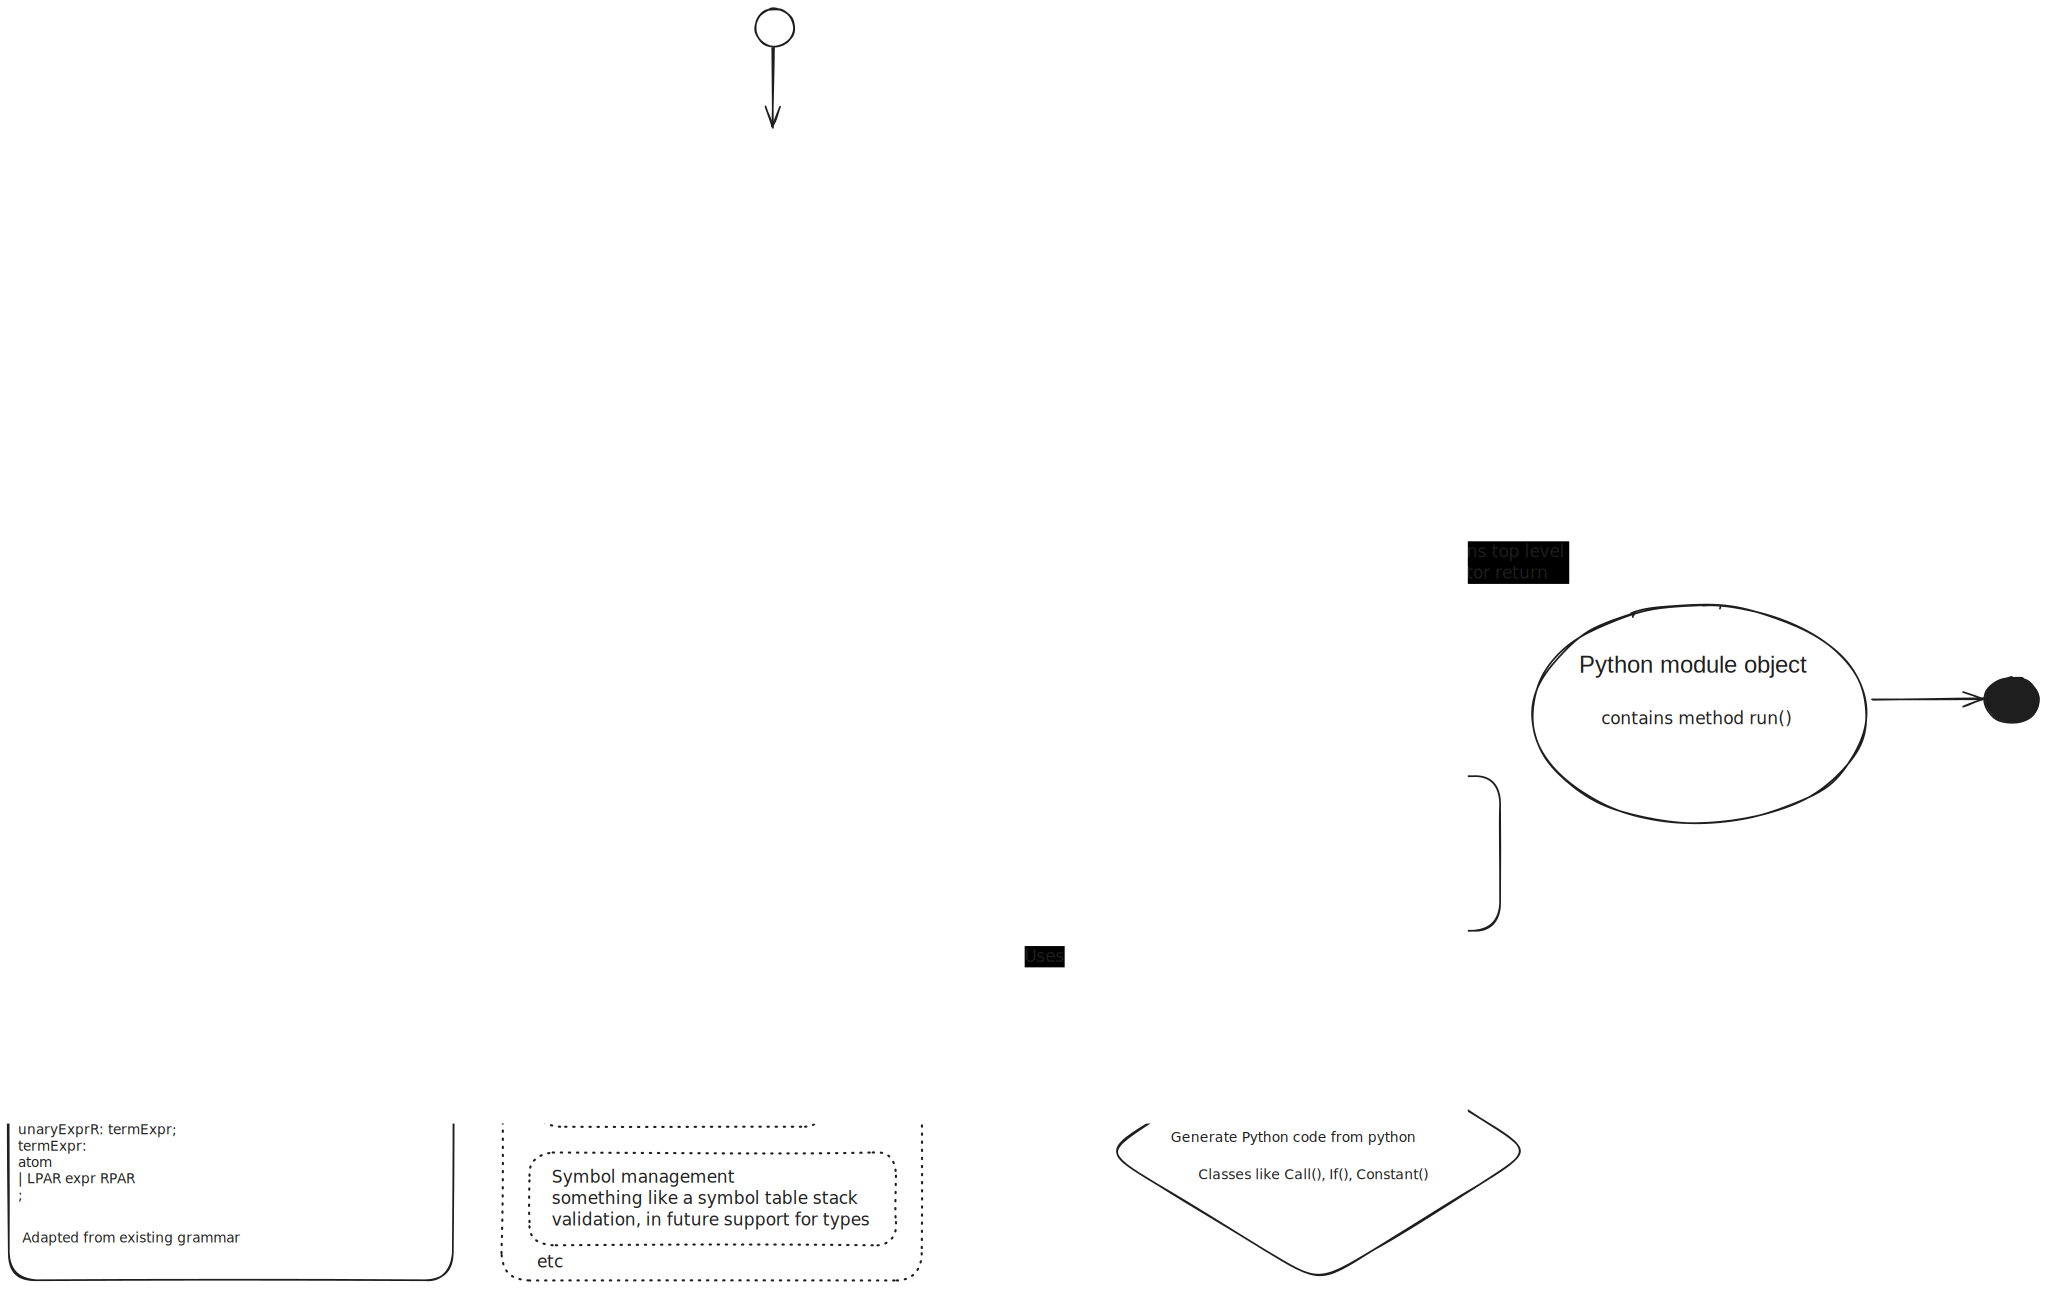
\includegraphics{img/expressions.svg}

\subsubsection{Visitor Pattern}
 From the parse tree, a visitor is generated—a component that traverses the parse tree. This visitor uses the visitor design pattern to execute operations based on the nodes of the parse tree. For the expression language, the visitor's primary role is to transform the parse tree into an Abstract Syntax Tree (AST) using Python’s ast module, which can then be executed or evaluated in a Python environment.

The following code snippet provides an example of how the visitor pattern is used to handle an AddExpr node in the parse tree:

\begin{verbatim}
    
def visitAddExpr(self, ctx: ExpressionsParser.AddExprContext):
    if ctx.left:
        op = ctx.op.children[0].symbol.type
        if op == ExpressionsParser.PLUS:
            name = Operator.ADD.value
        elif op == ExpressionsParser.MINUS:
            name = Operator.SUB.value
        else:
            raise ValueError(f"Unknown operator: {op}")
        identifier = self.get_symbol_table().get_identifier_for_name(name, "internal", "load")
        args = [self.visit(ctx.left), self.visit(ctx.right)]
        node = self.create_call_node(identifier, ctx.start.line, ctx.stop.line, args)
        return ExpressionArgument(node)

    return self.visitChildren(ctx)

\end{verbatim}

\subsubsection{Error Handling}

Syntax errors in the expressions are handled using ANTLR's error listeners. These listeners are customized to provide meaningful error messages that help in identifying and correcting syntax issues in the input expressions.

\subsection{Statements}

Handling variables and functions within expressions involves maintaining a symbol table where each variable's name and value are stored. Variables are parsed and evaluated through the visitor, which checks the symbol table to resolve their values during the execution of expressions.

 The symbol table keeps track of all symbols used in expressions. It ensures that each variable is correctly declared and used within its scope. Additionally, symbol transformation is employed to prevent collisions and ensure that variable names are unique within the global execution context.

 \subsection{Functions and Operators}

Implementing functions and operators in the Python version of the Ataccama Expression Language involves defining Python functions that correspond to each function and operator in the original language.

Each function from Ataccama’s language is mapped to a Python function. These functions handle various data types and perform the necessary computations or data manipulations as defined in the Ataccama language specifications.

Each operator is mapped to a function call with the operand(s) as the arguments. This allows for customizing behavior for arithmetic, logical, and comparison operations to closely align with how they function in the original implementation.

The reimplementation of the functions and operators constitutes a significant portion of the work, as the language supports a wide range of operations that need to be accurately translated to Python.

\subsection{Additional Features and Utilities}

In addition to the core features of the Ataccama Expression Language, several utilities and enhancements are implemented.

\subsubsection{Command Line Interface (CLI)}

A command-line interface is developed to allow users to interact with the expression evaluation engine directly. This CLI provides a simple way to input expressions and receive the output, making it easier to test and validate the implementation.

Running `poetry install` will make the `evaluate-records` script available.
`evaluate-records` can be used to evaluate records on a expression:

\begin{verbatim}
echo "John,25\nJohn,18" | evaluate-records "name == 'John' and
 age > 20" --record-format "name:STRING,age:INTEGER"
\end{verbatim}

\subsubsection{Expression Generator}

An expression generator is created to produce random expressions based on the grammar of the Ataccama Expression Language. This tool is useful for testing the parser and visitor components.

\section{Testing and Validation}
% Explain how you tested the reimplementation of DQ rules to ensure they work correctly and efficiently in local Python environments.

Testing and validation are critical components of the software development process, especially when reimplementing data quality (DQ) rules to ensure they perform as expected in local Python environments. For this project, we employ pytest with test parametrization to thoroughly test the Python implementation of Ataccama DQ rules.


Use of test Parametrization allows for running the same test function with different input values. It is particularly useful in this project for applying a wide array of test scenarios to the implemented functions to ensure comprehensive coverage and that the rules behave as intended across diverse data sets and conditions.

The primary focus during testing is to ensure that the reimplemented rules behave as similarly as possible to the Ataccama Expression Language. Tests are designed to validate both typical and edge-case scenarios, ensuring the rules are robust under various data conditions.

\subsection{Tool for Output Comparison}

To validate the accuracy of the reimplementation, we have developed a test suite that compares the outputs of our Python implementation against those generated by the original Ataccama ONE Expressions Java engine. This ensures that our implementation produces results consistent with the established behavior of the rules in the Ataccama environment.

This test suite can be run programatically using a script which the pytest test suite; the suite is using a fixture for running any expression that captures it and if enabled, saves it into a file. The script executes the tests and, for a subset of them, runs the same expressions in the Ataccama ONE Desktop environment. It then compares the outputs from both implementations and highlights any discrepancies.

The output can be used to identify any inconsistencies between the original and re-implemented rules, allowing for further refinement and debugging to ensure the rules are correctly implemented.

\section{Challenges and Resolutions}
% Discuss any challenges faced during the implementation and how they were resolved.

\subsection{Date formatting strings}
\paragraph{Problem}

One of the challenges encountered during the implementation was handling date formatting strings in the Ataccama Expression Language. The original language mirrors Java date formatting patterns, which are not directly compatible with Python’s datetime module. \cite{noauthor_datetimeformatter_nodate}

\paragraph{Resolution}

To address the date formatting issue, a mapping between Java and Python date formatting patterns was created. This mapping allows the Python implementation to interpret the date formatting strings correctly and convert them to the appropriate Python format.

To perform this mapping, a separate grammar with lexer and parser were added to parse the original date formatting string into pattern and text tokens. Pattern tokens are then converted using a lookup table.

\subsection{Multiline lambda functions}

\paragraph{Problem}

Another challenge was implementing multiline lambda functions in Python. The Ataccama Expression Language supports multiline lambda functions, which are not directly supported in Python. This required finding a workaround to enable multiline lambda functions in the Python implementation.

\paragraph{Resolution}

The solution involved defining full-fledged functions instead of using lambda expressions for multiline needs. To integrate these functions seamlessly and avoid namespace conflicts, we employed a symbol table that manages and mangles names dynamically. This approach ensures that all function names are unique and avoids identifier collisions within the Python environment, effectively replicating the flexibility of Ataccama's multiline lambdas within Python's syntactic constraints.
\subsection{Lookup Files}
\paragraph{Problem}

Ataccama's expressions can perform lookups against reference data stored in proprietary binary formats with sophisticated hashing strategies. This feature is crucial for validating data against predefined sets which are optimized for performance in Ataccama's native environment.
\paragraph{Solution}

To handle this, the proprietary lookup functionality was reimplemented in Python. This involved developing a method to read and interpret the binary format into a usable form in Python. Additionally, to mimic the fixed-size arithmetic and specialized hashing used by Ataccama, similar algorithms were implemented in Python, ensuring that the lookup performance remains efficient and consistent with the original implementation.
\subsection{Null Handling}
\paragraph{Problem}

Ataccama's functions and operators are designed to handle null values gracefully, often returning null or a neutral value when encountering nulls in expressions. This feature is essential for maintaining data integrity and ensuring robust data quality checks.
\paragraph{Solution}

The Python implementation adopted a similar approach to null handling. Custom operators and functions were developed to replicate the behavior of Ataccama's handling of nulls. For example, custom implementations of addition (+) and other operators were created to return null or appropriate neutral values when encountering null inputs. This ensures that the data quality rules continue to function predictably and effectively even when faced with incomplete or missing data.

This careful replication of functionality ensures that the Python version of Ataccama's DQ rules maintains the robustness and reliability of the original system, adhering closely to its operational logic and data handling practices.